% Created by tikzDevice version 0.12.6 on 2026-08-03 04:28:31
% !TEX encoding = UTF-8 Unicode
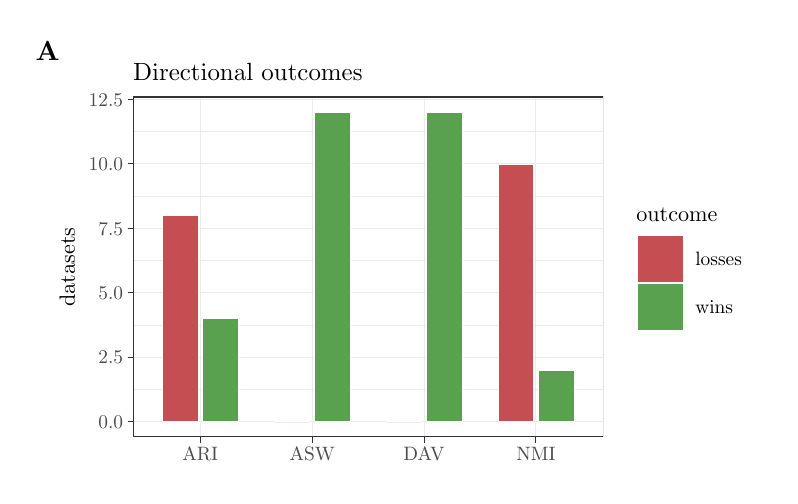
\begin{tikzpicture}[x=1pt,y=1pt]
\definecolor{fillColor}{RGB}{255,255,255}
\path[use as bounding box,fill=fillColor,fill opacity=0.00] (0,0) rectangle (268.03,161.83);
\begin{scope}
\path[clip] (  0.85,  1.74) rectangle (267.18,160.09);
\definecolor{drawColor}{RGB}{255,255,255}
\definecolor{fillColor}{RGB}{255,255,255}

\path[draw=drawColor,line width= 0.4pt,line join=round,line cap=round,fill=fillColor] (  0.85,  1.74) rectangle (267.18,160.09);
\end{scope}
\begin{scope}
\path[clip] ( 38.09, 13.93) rectangle (207.93,136.79);
\definecolor{fillColor}{RGB}{255,255,255}

\path[fill=fillColor] ( 38.09, 13.93) rectangle (207.93,136.79);
\definecolor{drawColor}{gray}{0.92}

\path[draw=drawColor,line width= 0.2pt,line join=round] ( 38.09, 31.15) --
	(207.93, 31.15);

\path[draw=drawColor,line width= 0.2pt,line join=round] ( 38.09, 54.42) --
	(207.93, 54.42);

\path[draw=drawColor,line width= 0.2pt,line join=round] ( 38.09, 77.69) --
	(207.93, 77.69);

\path[draw=drawColor,line width= 0.2pt,line join=round] ( 38.09,100.96) --
	(207.93,100.96);

\path[draw=drawColor,line width= 0.2pt,line join=round] ( 38.09,124.23) --
	(207.93,124.23);

\path[draw=drawColor,line width= 0.4pt,line join=round] ( 38.09, 19.52) --
	(207.93, 19.52);

\path[draw=drawColor,line width= 0.4pt,line join=round] ( 38.09, 42.79) --
	(207.93, 42.79);

\path[draw=drawColor,line width= 0.4pt,line join=round] ( 38.09, 66.05) --
	(207.93, 66.05);

\path[draw=drawColor,line width= 0.4pt,line join=round] ( 38.09, 89.32) --
	(207.93, 89.32);

\path[draw=drawColor,line width= 0.4pt,line join=round] ( 38.09,112.59) --
	(207.93,112.59);

\path[draw=drawColor,line width= 0.4pt,line join=round] ( 38.09,135.86) --
	(207.93,135.86);

\path[draw=drawColor,line width= 0.4pt,line join=round] ( 62.35, 13.93) --
	( 62.35,136.79);

\path[draw=drawColor,line width= 0.4pt,line join=round] (102.79, 13.93) --
	(102.79,136.79);

\path[draw=drawColor,line width= 0.4pt,line join=round] (143.23, 13.93) --
	(143.23,136.79);

\path[draw=drawColor,line width= 0.4pt,line join=round] (183.66, 13.93) --
	(183.66,136.79);
\definecolor{drawColor}{RGB}{255,255,255}
\definecolor{fillColor}{RGB}{89,161,79}

\path[draw=drawColor,line width= 0.2pt,fill=fillColor] (184.47, 19.52) rectangle (197.41, 38.13);

\path[draw=drawColor,line width= 0.2pt,fill=fillColor] ( 63.16, 19.52) rectangle ( 76.10, 56.75);

\path[draw=drawColor,line width= 0.2pt,fill=fillColor] (103.60, 19.52) rectangle (116.54,131.21);

\path[draw=drawColor,line width= 0.2pt,fill=fillColor] (144.04, 19.52) rectangle (156.98,131.21);
\definecolor{fillColor}{RGB}{196,78,82}

\path[draw=drawColor,line width= 0.2pt,fill=fillColor] (169.92, 19.52) rectangle (182.86,112.59);

\path[draw=drawColor,line width= 0.2pt,fill=fillColor] ( 48.61, 19.52) rectangle ( 61.55, 93.98);

\path[draw=drawColor,line width= 0.2pt,fill=fillColor] ( 89.04, 19.52) rectangle (101.98, 19.52);

\path[draw=drawColor,line width= 0.2pt,fill=fillColor] (129.48, 19.52) rectangle (142.42, 19.52);
\definecolor{drawColor}{gray}{0.20}

\path[draw=drawColor,line width= 0.4pt,line join=round,line cap=round] ( 38.09, 13.93) rectangle (207.93,136.79);
\end{scope}
\begin{scope}
\path[clip] (  0.00,  0.00) rectangle (268.03,161.83);
\definecolor{drawColor}{gray}{0.30}

\node[text=drawColor,anchor=base east,inner sep=0pt, outer sep=0pt, scale=  0.70] at ( 34.49, 17.11) {0.0};

\node[text=drawColor,anchor=base east,inner sep=0pt, outer sep=0pt, scale=  0.70] at ( 34.49, 40.38) {2.5};

\node[text=drawColor,anchor=base east,inner sep=0pt, outer sep=0pt, scale=  0.70] at ( 34.49, 63.64) {5.0};

\node[text=drawColor,anchor=base east,inner sep=0pt, outer sep=0pt, scale=  0.70] at ( 34.49, 86.91) {7.5};

\node[text=drawColor,anchor=base east,inner sep=0pt, outer sep=0pt, scale=  0.70] at ( 34.49,110.18) {10.0};

\node[text=drawColor,anchor=base east,inner sep=0pt, outer sep=0pt, scale=  0.70] at ( 34.49,133.45) {12.5};
\end{scope}
\begin{scope}
\path[clip] (  0.00,  0.00) rectangle (268.03,161.83);
\definecolor{drawColor}{gray}{0.20}

\path[draw=drawColor,line width= 0.4pt,line join=round] ( 36.09, 19.52) --
	( 38.09, 19.52);

\path[draw=drawColor,line width= 0.4pt,line join=round] ( 36.09, 42.79) --
	( 38.09, 42.79);

\path[draw=drawColor,line width= 0.4pt,line join=round] ( 36.09, 66.05) --
	( 38.09, 66.05);

\path[draw=drawColor,line width= 0.4pt,line join=round] ( 36.09, 89.32) --
	( 38.09, 89.32);

\path[draw=drawColor,line width= 0.4pt,line join=round] ( 36.09,112.59) --
	( 38.09,112.59);

\path[draw=drawColor,line width= 0.4pt,line join=round] ( 36.09,135.86) --
	( 38.09,135.86);
\end{scope}
\begin{scope}
\path[clip] (  0.00,  0.00) rectangle (268.03,161.83);
\definecolor{drawColor}{gray}{0.20}

\path[draw=drawColor,line width= 0.4pt,line join=round] ( 62.35, 11.93) --
	( 62.35, 13.93);

\path[draw=drawColor,line width= 0.4pt,line join=round] (102.79, 11.93) --
	(102.79, 13.93);

\path[draw=drawColor,line width= 0.4pt,line join=round] (143.23, 11.93) --
	(143.23, 13.93);

\path[draw=drawColor,line width= 0.4pt,line join=round] (183.66, 11.93) --
	(183.66, 13.93);
\end{scope}
\begin{scope}
\path[clip] (  0.00,  0.00) rectangle (268.03,161.83);
\definecolor{drawColor}{gray}{0.30}

\node[text=drawColor,anchor=base,inner sep=0pt, outer sep=0pt, scale=  0.70] at ( 62.35,  5.51) {ARI};

\node[text=drawColor,anchor=base,inner sep=0pt, outer sep=0pt, scale=  0.70] at (102.79,  5.51) {ASW};

\node[text=drawColor,anchor=base,inner sep=0pt, outer sep=0pt, scale=  0.70] at (143.23,  5.51) {DAV};

\node[text=drawColor,anchor=base,inner sep=0pt, outer sep=0pt, scale=  0.70] at (183.66,  5.51) {NMI};
\end{scope}
\begin{scope}
\path[clip] (  0.00,  0.00) rectangle (268.03,161.83);
\definecolor{drawColor}{RGB}{0,0,0}

\node[text=drawColor,rotate= 90.00,anchor=base,inner sep=0pt, outer sep=0pt, scale=  0.80] at ( 17.05, 75.36) {datasets};
\end{scope}
\begin{scope}
\path[clip] (  0.00,  0.00) rectangle (268.03,161.83);
\definecolor{fillColor}{RGB}{255,255,255}

\path[fill=fillColor] (215.93, 48.25) rectangle (265.18,102.47);
\end{scope}
\begin{scope}
\path[clip] (  0.00,  0.00) rectangle (268.03,161.83);
\definecolor{drawColor}{RGB}{0,0,0}

\node[text=drawColor,anchor=base west,inner sep=0pt, outer sep=0pt, scale=  0.80] at (219.93, 91.95) {outcome};
\end{scope}
\begin{scope}
\path[clip] (  0.00,  0.00) rectangle (268.03,161.83);
\definecolor{fillColor}{RGB}{255,255,255}

\path[fill=fillColor] (219.93, 69.60) rectangle (237.27, 86.94);
\definecolor{drawColor}{RGB}{255,255,255}
\definecolor{fillColor}{RGB}{196,78,82}

\path[draw=drawColor,line width= 0.2pt,fill=fillColor] (220.21, 69.88) rectangle (236.99, 86.66);
\end{scope}
\begin{scope}
\path[clip] (  0.00,  0.00) rectangle (268.03,161.83);
\definecolor{fillColor}{RGB}{255,255,255}

\path[fill=fillColor] (219.93, 52.25) rectangle (237.27, 69.60);
\definecolor{drawColor}{RGB}{255,255,255}
\definecolor{fillColor}{RGB}{89,161,79}

\path[draw=drawColor,line width= 0.2pt,fill=fillColor] (220.21, 52.54) rectangle (236.99, 69.31);
\end{scope}
\begin{scope}
\path[clip] (  0.00,  0.00) rectangle (268.03,161.83);
\definecolor{drawColor}{RGB}{0,0,0}

\node[text=drawColor,anchor=base west,inner sep=0pt, outer sep=0pt, scale=  0.70] at (241.27, 75.86) {losses};
\end{scope}
\begin{scope}
\path[clip] (  0.00,  0.00) rectangle (268.03,161.83);
\definecolor{drawColor}{RGB}{0,0,0}

\node[text=drawColor,anchor=base west,inner sep=0pt, outer sep=0pt, scale=  0.70] at (241.27, 58.51) {wins};
\end{scope}
\begin{scope}
\path[clip] (  0.00,  0.00) rectangle (268.03,161.83);
\definecolor{drawColor}{RGB}{0,0,0}

\node[text=drawColor,anchor=base west,inner sep=0pt, outer sep=0pt, scale=  0.90] at ( 38.09,142.78) {Directional outcomes};
\end{scope}
\begin{scope}
\path[clip] (  0.00,  0.00) rectangle (268.03,161.83);
\definecolor{drawColor}{RGB}{0,0,0}

\node[text=drawColor,anchor=base,inner sep=0pt, outer sep=0pt, scale=  1.00] at (  7.20,150.08) {\bfseries A};
\end{scope}
\end{tikzpicture}
